\documentclass[UTF8]{ctexart}

\usepackage[linesnumbered,boxed,ruled,commentsnumbered]{algorithm2e}
\usepackage{bm}
\usepackage{graphicx}
\usepackage{float}
\usepackage[bookmarks=true]{hyperref}
\usepackage{amsmath}
\begin{document}
\title{计网大作业——基于中央定位服务器的P2P聊天系统}
\author{陈昭熹 2017011552}
\maketitle
\tableofcontents
\newpage

\section{需求分析}
本次大作业中,要求实现一个基于中央定位服务器的P2P网络聊天系统,该系统主体结构如下所示:

用户将通过中央服务器来登录、离线、查询好友通信IP,实际通信数据流通过Peer to Peer的隧道实现,不需要服务器参与。

本次实验后端使用Python实现,前端使用PyQt5.

本次实验我实现了如下功能:
\begin{itemize}
    \item[\textbf{必做部分}] 
    \item 账号登录上线/下线
    \item 维护通讯录,查询好友是否在线
    \item P2P文字通信(TCP)
    \item 文件传输(10M以上)
    \item 友好的GUI
    \item[\textbf{选做部分}]
    \item 语音和视频通话
    \item 创新点:路由式线程管理 
\end{itemize}

\section{系统架构}\label{arch}
系统架构如下所示:
\begin{figure}[H]
    \centering
    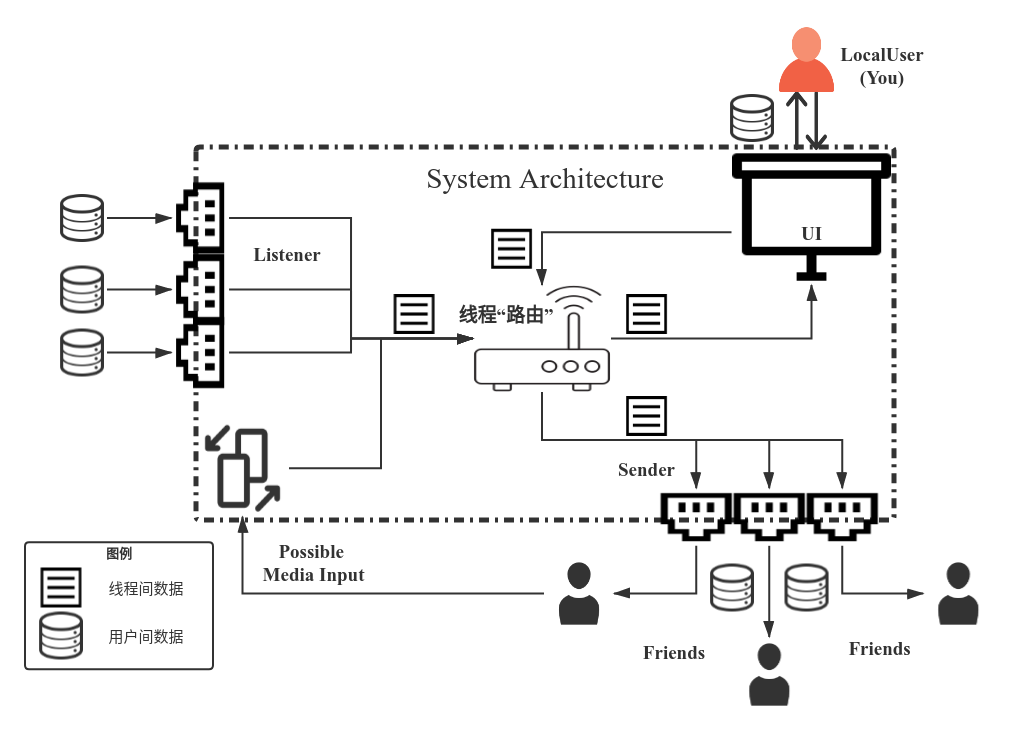
\includegraphics[scale=0.33]{myqq.png}
    \caption{系统架构}
\end{figure}

\subsection{基础收发模式}

用户之间的通信采取报头+数据的形式,在每次通信之前首先由发送方发送报头,在接收方接收到后将其解封装,开辟好相应的内存空间,并告知进程下各线程后返回ACK确定准备接受。再由发送方将原始数据发送过来,进行接受处理。

每个客户端成功登陆后,会自动启动监听线程,等待连接,即Listener\ref{listener}

在用户操作中,每向一个用户发送消息时,会自动检测是否建立了连接,否则会向目标IP启动发送线程,请求连接,即Sender\ref{sender}

\subsubsection{Sender}\label{sender}
一个发送线程即一个面向目标IP的TCP套接字,成功建立连接后,该线程从缓存中不断取出从线程“路由”发来的数据,并根据数据格式和内容,首先将数据报报头通过套接字发送给目标端,等待ACK,接收到确认后将数据发送出去,表示为状态机如下:
\begin{figure}[H]
    \centering
    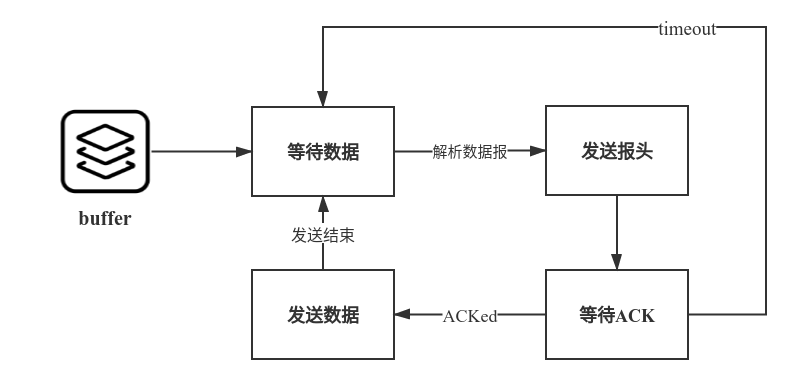
\includegraphics[scale=0.4]{senderstate.png}
    \caption{Sender状态机}
\end{figure}


\subsubsection{Listener}\label{listener}
一个监听线程即一个绑定在本地的TCP监听套接字,本次实验使用本地的9876端口。每当监听到一个新的连接请求,将建立的TCP连接套接字和对应的数据接受功能放入新的线程运行,并重新回到监听状态,表示为状态机如下:
\begin{figure}[H]
    \centering
    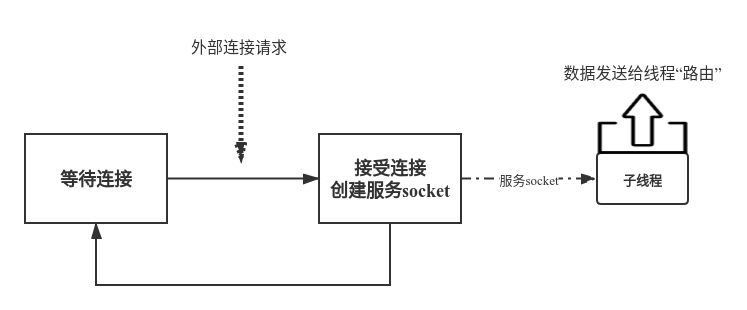
\includegraphics[scale=0.4]{listenerstate.png}
    \caption{Listener状态机}
\end{figure}

\subsection{进程通信协议}\label{progress}
所谓进程通信协议即用户与用户之间的数据通信协议,用于统一同一网络下的不同客户端之间的数据报格式。
如上所述,由于采取报头+数据的方式进行通信,下面给出\textbf{进程间数据报报头格式}定义如下:
\begin{table}[H]
    \centering
    \begin{tabular}{cc}
        \hline
        字段名称 & 数据内容 \\
        \hline
        sender\_id & 发送方学号\\
        recver\_id & 接收方学号\\
        data\_type & 数据类型\\
        date & 时间戳\\
        optional & 可选字段(包含以下内容)\\
        file\_name(optional) & 文件名\\
        file\_size(optional) & 文件大小(包含分片)\\
        charset(optional) & 编码方式\\
        command\_type(optional) & 命令类型\\
        \hline
    \end{tabular}
\end{table}

利用TCP通信的可靠性,使用上述数据报协议可以安全可靠地进行数据传输,后续数据无需进行包装,只需要根据分片和大小进行发送和接受即可。



\subsection{线程通信协议}\label{thread}

为了保持系统各个模块并发同步地安全运行,需要对于程序下的线程之间通信建立协议,避免直接访问内存式的数据交换,导致段错误。\textbf{线程之间通信数据格式与协议}如下:
\begin{table}[H]
    \centering
    \begin{tabular}{cc}
        \hline
        字段名称 & 数据内容 \\
        \hline
        sender\_type & 发送者线程类型\\
        recver\_type & 接受者线程类型\\
        data\_type & 数据类型\\
        data & 原始数据 \\
        optional & 可选字段(包含以下内容)\\
        destination & 发送目的地(即目标IP)\\
        command\_type&命令类型\\
        \hline
    \end{tabular}
\end{table}

系统中同时运行着多种不同的线程,诸如监听socket、发送socket、用户界面、视频流处理等,每个线程视为一个worker,具备不同的类型,通过独立线程下的一个交换机来完成内部通信和数据交换,具体设计下一节将会详细说明\ref{router},这里给出上述通信协议中不同字段的值和对应语义:
\begin{table}[H]
    \centering
    \begin{tabular}{ccc}
        \hline
        字段名称 & 可能取值 & 语义\\
        \hline
        & 1 & 监听Socket\\
        线程&2&发送Socket\\
        类型&3&与中央服务器的连接线程\\
        &4&GUI线程\\
        \hline
        &1&命令\\
        数据&2&纯文本\\
        类型&3&文件\\
        &4&视频\\
        \hline
        &1&登录\\
        &2&建立P2P连接\\
        命令&3&断开P2P连接\\
        类型&4&下线\\
        &5&查询好友状态\\
        &6&好友请求\\
        &7&拒绝好友请求\\
        \hline
    \end{tabular}
\end{table}

\subsection{线程"路由"——基于Producter-Consumer模式}\label{router}
本节阐述如何在这个复杂系统中进行安全的线程管理,并且保证高效的系统吞吐率。
事实上,在高并发情况下,一个客户端下会运行数十个子线程,为了提高处理速度,并且保证线程安全,需要统一管理线程。但是简单的使用线程池等方式又无法对于一些数据交换频率高的线程进行优化管理。受到计算机网络课堂学习的内容的启发,一个客户端下的若干线程正如同一个网络中的若干端系统,如何让网络中的端系统高效进行数据交换也就可以用类似的思路管理线程,使用一个类似网络中的路由的结构能够让线程之间进行高效安全的通信。

使用上一节介绍的良好的线程通信协议,基于Producter-Consumer模式,单独运行一个$router$线程,管理所有的子线程,就好像其他子线程均通过一根网线连到了该线程,即线程“路由”。为什么叫路由而不是交换机,原因在于设计过程中将一部分的复杂度放在了该线程路由上,而非端线程上,让其根据数据内容进行针对性数据发送,而不是广播,提高效率。

类似计算机网络中端系统+路由组网的过程,在线程“路由”中,使用Thread-ID作为线程唯一标示,使用互斥的线程池存储子线程句柄。该线程“路由”工作模式如下:
\begin{itemize}
    \item[\textbf{接受数据}]通过定义外部接口recv供其他线程调用,将Producter线程发布的数据视为一个task缓存到$router$线程的优先级队列中。每一个数据均用上一节中的数据通信协议\ref{thread}进行封装。
    \item[\textbf{接入子线程/组网}]通过定义内部接口attach,将一个Consumer子线程接入线程“路由”,该子线程能够被动得接受线程路由发送给其的数据,但没有发送权限。
    \item[\textbf{退出路由/断网}]通过定义内部接口detach,将某一Consumer子线程结束并销毁句柄,回收内存,并将该子线程与线程“路由”的连接断开。
    \item[\textbf{路由}]循环执行。通过定义内部接口routing,作为一个守护线程运行在系统后端,从task优先级队列中取出首个task,根据协议解封装,并根据其中的recver\_type等字段将其发送给相应的Consumer子线程。
\end{itemize}

该线程“路由”作为本系统的组织核心,在系统结构中的作用和位置已经在前文\ref{arch}给出。


\section{功能设计}
下面分为必做和选做两个部分介绍具体功能实现思路。

\subsection{必做部分}
本部分的网络连接和套接字管理均建立在\ref{listener}\ref{sender}\ref{router}基础上,仅介绍具体功能的实现流程。
\subsubsection{账号上线下线}
中央服务器的指令集已经在作业要求中给出。在客户端启动时,首先向中央服务器发起连接(IP:166.111.140.57,port:8000),当用户点击登录按钮时,将用户的学号按照指令集的格式(由于\textbf{密码默认为net2019},因此就没有增加密码输入框,在一个实用的聊天工具中密码应当是存在的)发送给中央服务器进行验证,验证成功后跳转到主界面。在用户名验证时,加入正则表达式约束,防止输入不合规则的学号。
\subsubsection{通讯录维护}
进入主界面后,通过点击Contacts右侧的添加好友按钮,弹出窗口,输入好友学号进行添加。系统首先向中央服务器查询好友学号,若不存在则会提示查无此人,若不在线则会提示连接拒绝,否则会通过发送线程向好友发送好友请求。此时好友端接收到请求后由后端发起,自动弹窗进行好友确认,若点击拒绝,则己方显示拒绝,否则会显示添加成功,在通讯录中自动更新好友学号的一栏。值得注意的是根据好友名字颜色可以区分其在线状态:\textbf{灰色}-不在线;\textbf{绿色}-在线。
\subsubsection{P2P文字通信}
使用前文描述的用户间通信协议\ref{progress},可以实现用户之间的P2P纯文本通信。通过在通信录选择联系人,在输入框中输入文字,选择发送功能为text,点击发送即可通过发送线程将文字发给好友。消息框中绿色背景为自己发送的信息,白色背景为对方发给自己的信息

\subsubsection{文件传输}
同样使用前文描述的用户间通信协议\ref{progress},可以较好的实现用户之间的大于10M的文件传输,传输速度视网络状况而定。在相应人的聊天窗口下,选择发送功能为file,在弹出的文件浏览窗中选择对应文件,即可开始传输。在好友端会保存在当前运行目录下,文件名增加recved\_前缀。
\subsubsection{GUI}
用户界面使用PyQt5予以实现,并且基于信号-槽进行了线程安全的设计。主窗口界面类似电脑端微信,各按钮功能一目了然,在此不多赘述。值得注意的是视频聊天点击之后需要稍微等待一会,等待声卡、摄像头等硬件启动。若长时间未弹出通话窗口,可能是由于硬件启动失败或对方拒绝连接。请查看命令行输出。

\subsection{选做部分}
选做部分的网络通信设计独立于前述,未使用\ref{sender}所述的发送线程。主要是由于视频流、音频流需要解码、压缩等,同时对带宽占用较大,因此单独处理。
\subsubsection{语音视频通话}
音视频通话使用独立设计的套接字clientMedia和serverMedia,分别对应音视频发送和接收。类似于前面的Listener\ref{listener},serverMedia在客户端一开始就运行起来,等待他人连接请求。值得一提的是由于带宽有限,本套接字监听的连接上限设置为1。在用户点击聊天界面的video并点击发送后,会自动向目标端发送视频连接请求,若同意请求,则近端会接收到从远端返回的视频连接(由远端运行clientMedia连接近端serverMedia),并自动弹窗显示对方视频。此时若对方也想查看你的视频,请等待对方发送的视频连接请求。

在底层处理上,为了保证传输质量,音视频数据流分别在两个套接字管理的TCP连接中进行。音频流使用PyAudio库获得,\textbf{此处应注意不同端系统声卡表现不一样,使用前请检查硬件设备,否则会导致连接无法建立},通过码率44100,双通道进行传输。在采样过程中,采用了通过阈值进行降噪的策略。如果发现连接中没有声音,请调高系统音量,调整麦克风。

视频流通过opencv的videocapture获得,视频采样大小为$640\times480\times3$三通道彩色图像。为了保证传输速率,使用zlib库的压缩来对原始图像进行编码压缩。在数据流传输过程中采取分块策略,首先通过报头让接收方得知压缩后的单帧视频大小,并准备好分块接受。通过定义CHUNK来约束最大数据块,并通过循环将该帧视频通过TCP连接连续发送出去。接收方用类似的方法进行循环接受,解压缩,并且通过numpy相关功能拼接成完整图片。

实验过程中发现,实际上仅仅通过CPU处理,实时的视频压缩与解压缩并不能高速实时实现,还不如直接发送原始图片来的流程。但最终还是保留了压缩设计。
\subsubsection{线程"路由"设计}
如前所述\ref{router},此处不再赘述。
\section{结果}

\end{document}